\documentclass[11pt]{report}
\usepackage[margin=1.1in]{geometry}
\usepackage[utf8]{inputenc}
\usepackage[italian]{babel}
\usepackage{amssymb} 
\usepackage{amsmath}
\usepackage{amsthm}
\usepackage{thmtools}
\usepackage{pdfpages}
\usepackage{hyperref}

\setcounter{tocdepth}{3}
\setcounter{secnumdepth}{3}

\newcommand{\desctotoc}[1]{%
  \addtocontents{toc}{\medskip\noindent\detokenize{#1}\leavevmode\par\medskip}
}

\begin{document}
\title{Appunti su \emph{Struttura del calcolatore}}
\author{Gabriele Frassi}
\date{A.A 2020-2021 - Primo semestre}
\maketitle

\small\tableofcontents\normalsize

\chapter{Unimap}
\small
\begin{enumerate}
\item \textbf{Mer 25/11/2020 10:45-12:00 (1:30 h)} esercitazione: Esercizi di descrizione e sintesi di reti sequenziali sincronizzate. (GIOVANNI STEA)
\item \textbf{Gio 26/11/2020 10:45-12:45 (2:0 h)} lezione: Il calcolatore visto come un insieme di moduli interconnessi: processore, spazio di memoria e spazio di I/O. Visione funzionale del processore didattico sEP8 (8 bit simple Educational Processor): i registri, le istruzioni, inizializzazione al reset. Modalità di indirizzamento degli operandi. Linguaggio Assembler e linguaggio macchina. Formato delle istruzioni. (GIOVANNI STEA)
\item \textbf{Ven 27/11/2020 15:00-17:00 (2:0 h)} esercitazione: (in copresenza con ing. Raffaele Zippo): svolgimento di esercizi di descrizione e sintesi di reti sequenziali e combinatorie in ambiente Verilog. (GIOVANNI STEA)
\item \textbf{Mar 01/12/2020 11:45-13:45 (2:0 h)} lezione: descrizione del calcolatore: memoria, spazio di I/O, processore. Descrizione dei registri del processore. Letture e scritture in memoria e nello spazio di I/O. Descrizione della fase di reset e di fetch in Verilog. (GIOVANNI STEA)
\item \textbf{Mer 02/12/2020 10:45-12:45 (2:0 h)} lezione: Descrizione del processore: fase di esecuzione. Interfacce: visione funzionale. Interfacce con e senza handshake. Accesso a controllo di programma. (GIOVANNI STEA)
\item \textbf{Gio 03/12/2020 10:45-12:45 (2:0 h)} lezione: Interfacce parallele con e senza handshake, ingresso ed uscita. Trasmissione seriale start/stop. Interfaccia seriale. (GIOVANNI STEA)
\item \textbf{Ven 04/12/2020 15:00-17:00 (2:0 h)} esercitazione: (in copresenza con ing. Raffaele Zippo). Svolgimento di esercizi di descrizione di reti complesse al calcolatore. (GIOVANNI STEA)
\item \textbf{Mer 09/12/2020 10:45-12:45 (2:0 h)} lezione: Descrizione del trasmettitore e ricevitore seriale. Conversione analogico/digitale e digitale/analogica. Convertitore D/A ed interfaccia di conversione. (GIOVANNI STEA)
\item \textbf{Gio 10/12/2020 10:45-12:45 (2:0 h)} lezione: Convertitore analogico/digitale e relativa interfaccia di conversione. Chiusura del corso. (GIOVANNI STEA)
\end{enumerate}
\normalsize


\part{Struttura di un calcolatore}
\chapter{Giovedì 26/11/2020}
\desctotoc{\small\begin{itemize}
\item Recap sul calcolatore di Von Neumann: sottosistema di I/O, memoria principale e processore (sEP8).
\item Calcolatore visto dal programmatore,
\item Linguaggio Assembler per il processore sEP8: opcode, formati.
\item Architettura del calcolatore: processore e sottosistema di I/O visti come RSS, memoria principale vista come una RSA.
\end{itemize}\normalsize}
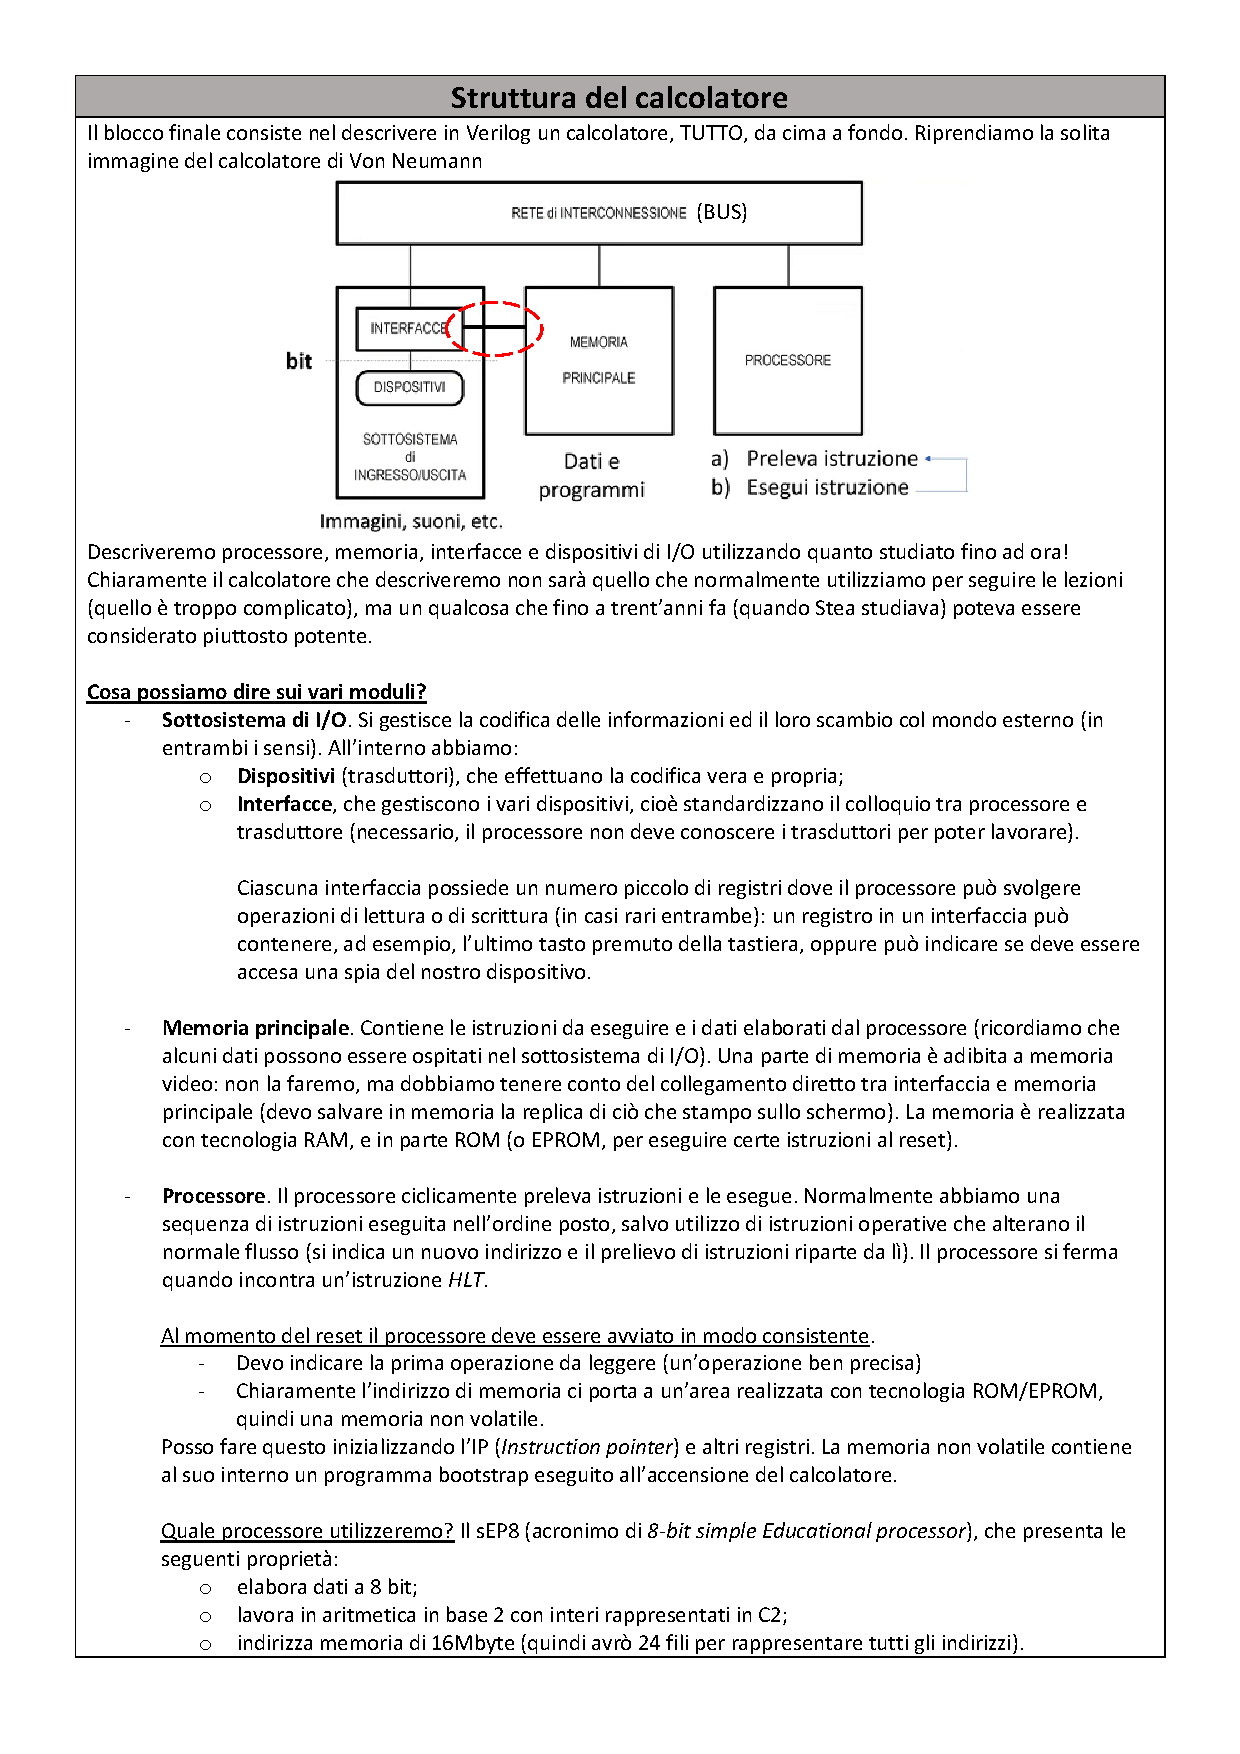
\includepdf[pagecommand={\thispagestyle{plain}},scale=0.92,pages=-]{pdf/calcolatore1}
\section{Ricapitoliamo sui formati}
I formati non vanno imparati a memoria, ma ricordati mediante la logica.
\paragraph{Quanti sono gli operandi?} Otto, lo capisco dal numero di bit dedicati al formato (3).
\paragraph{Quali sono i formati?} Seguire la scaletta.
\begin{itemize}
\item \textbf{Primo formato} (F0): quello dove la vita è più semplice, non dobbiamo andare a recuperare nessun operando.
\item \textbf{Terzo e quarto formato} (F2, F3): registri puntatore, rispettivamente in source e destination. L'altro operando è un registro.
\item \textbf{Quinto formato} (F4): costante in source. L'altro operando è registro.
\item \textbf{Sesto e settimo formato} (F5, F6): indirizzamento diretto, rispettivamente in source e dest. L'altro operando è registro.
\item \textbf{Ottavo formato} (F7): istruzioni di salto (sia quello condizionato che non). L'operando è registro.
\item \textbf{Secondo formato} (F1): varie ed eventuali, precisamente istruzioni IN/OUT o modifica di registri a 24bit (i registri puntatore). Lo si lascia in fondo nel ragionamento.
\end{itemize}

\chapter{Martedì 01/12/2020}
\desctotoc{\small\begin{itemize}
\item Spazio di memoria.
\item Spazio di I/O.
\item Processore. 
\item Fasi del processore: reset iniziale, fase di fetch, fase di esecuzione, stato di blocco.
\item Letture e scritture in memoria: temporizzazione ed esempio Verilog.
\item Lettura e scritture nel sottosistema di I/O: temporizzazione ed esempio Verilog.
\item Sottoprogrammi per operazioni di lettura o scrittura in memoria (su 1, 2, 3, 4 byte).
\item Inizio della descrizione in Verilog del processore: reset, functions di supporto (valid$\_$fetch, first$\_$execution$\_$state, alu$\_$result, alu$\_$flag, jmp$\_$condition), fase di fetch.
\end{itemize}\normalsize}
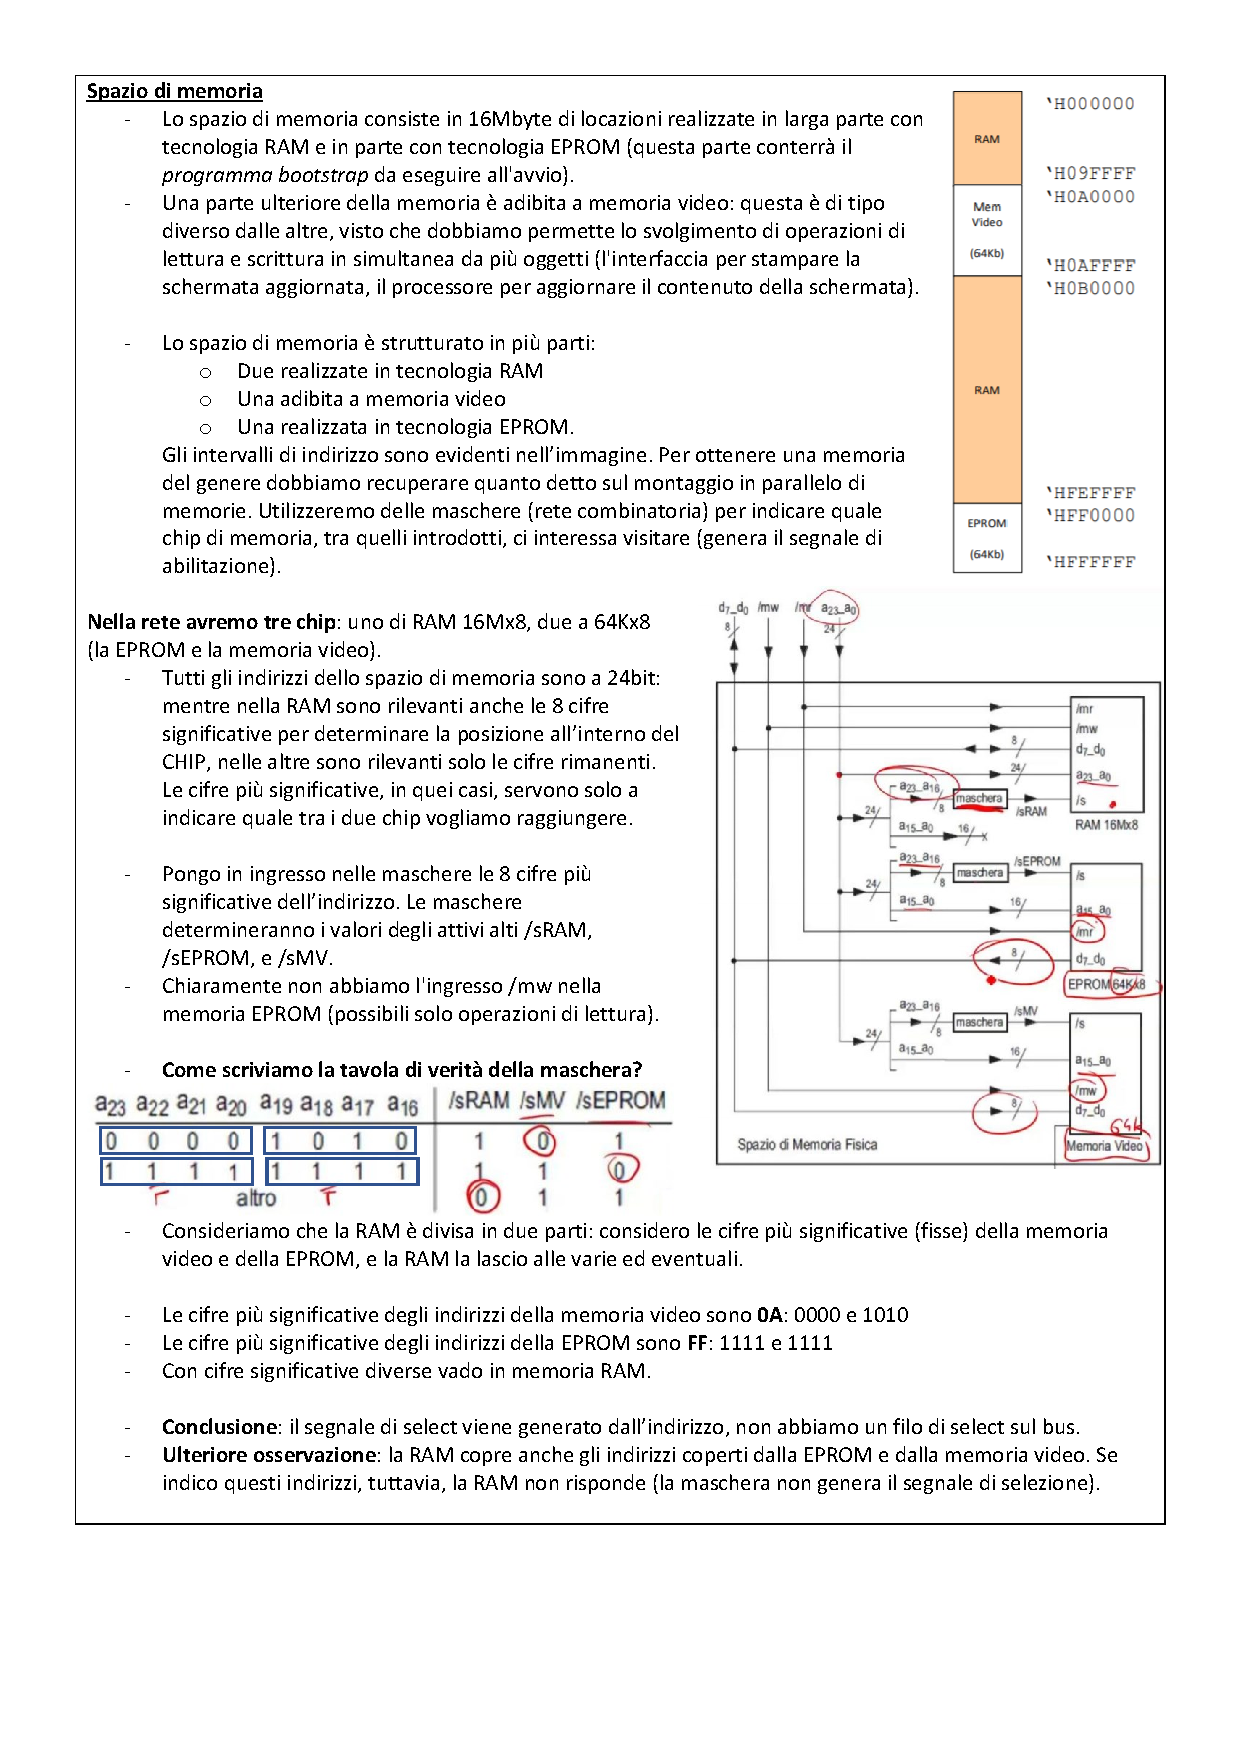
\includepdf[pagecommand={\thispagestyle{plain}},scale=0.92,pages=-]{pdf/calcolatore2}

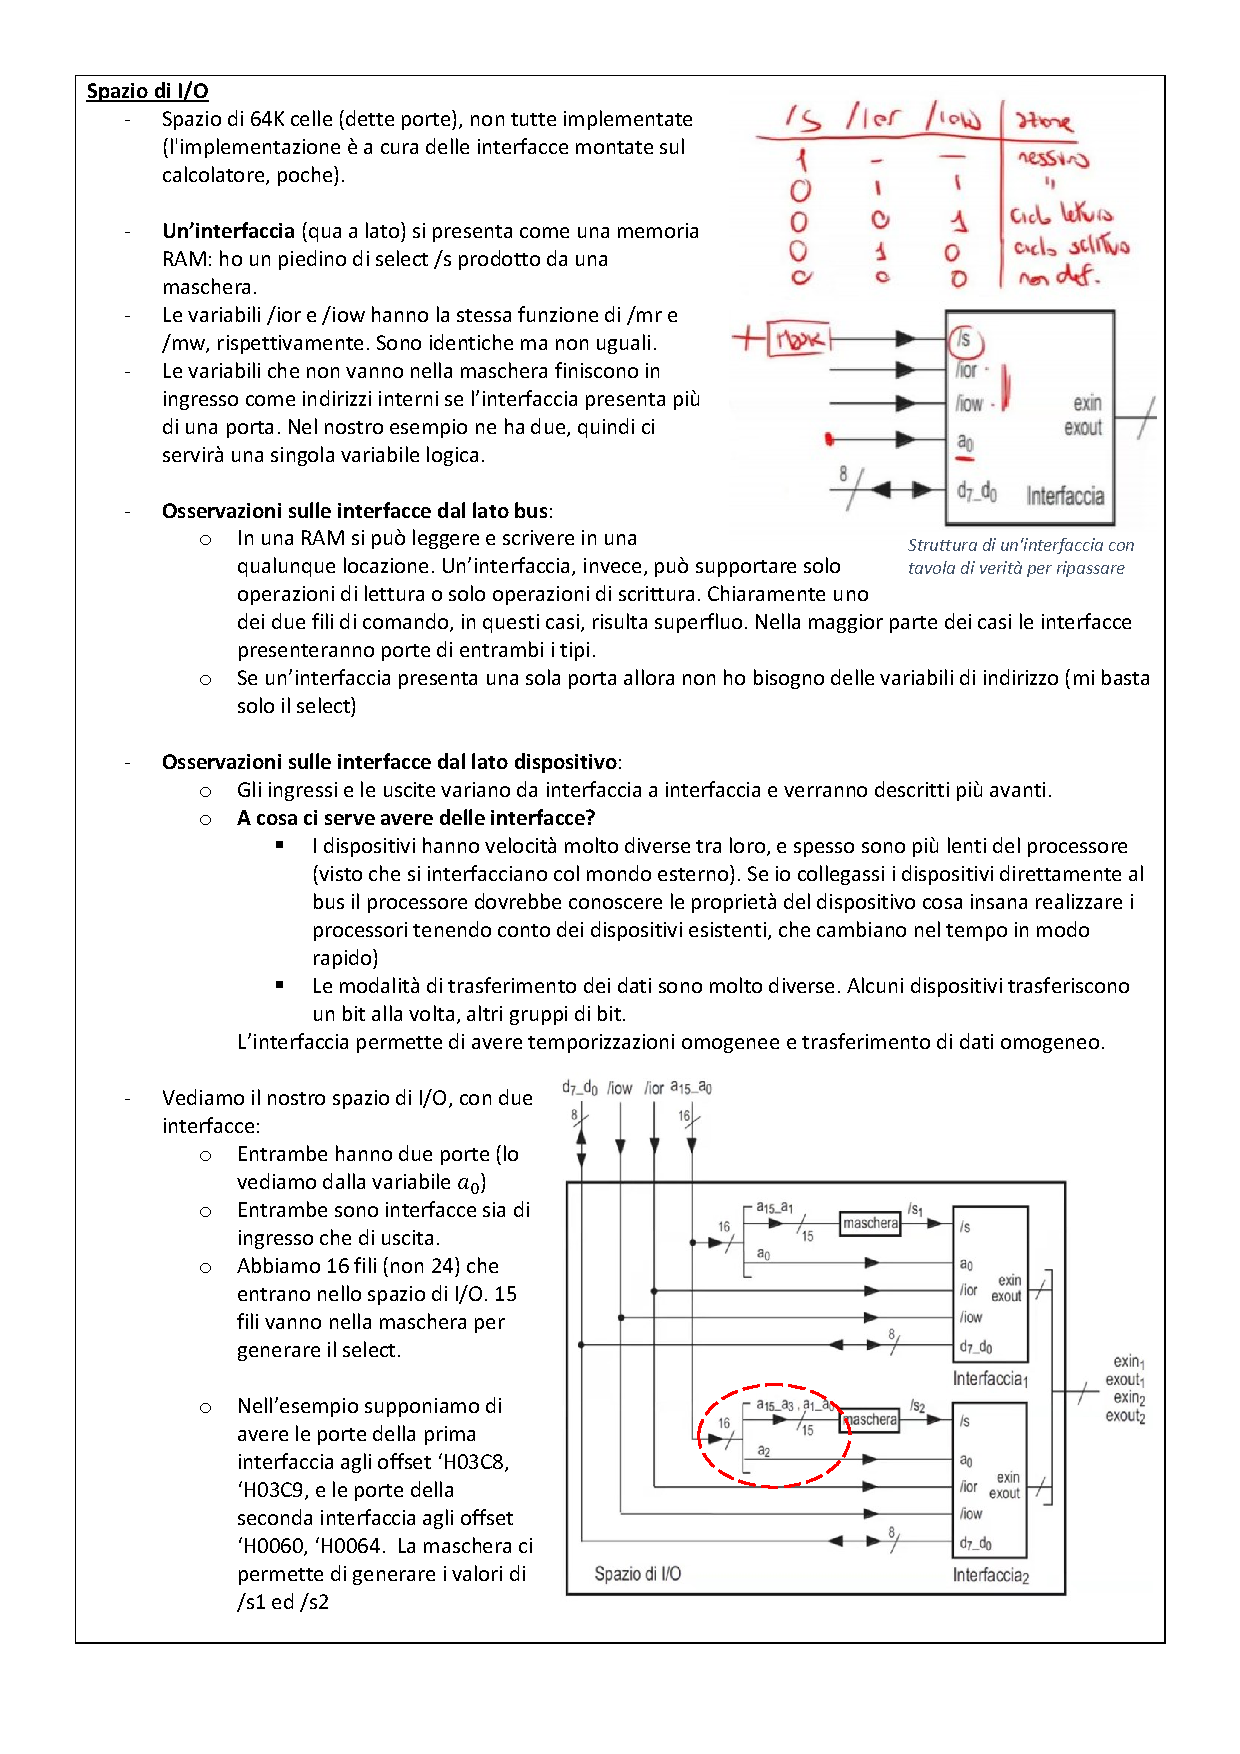
\includepdf[pagecommand={\thispagestyle{plain}},scale=0.92,pages=-]{pdf/calcolatore3}
\section{Ricapitoliamo sulle operazioni di lettura e scrittura...}
\subsection{Memoria principale}
\begin{center}
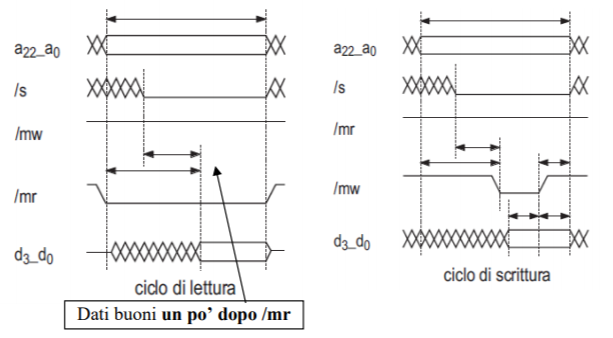
\includegraphics{img/231.PNG}
\end{center}
\begin{itemize}
\item Quando scriviamo il codice Verilog dobbiamo tenere conto di quanto già visto nello spiegare la temporizzazione di scrittura e lettura in una memoria RAM statica:
\begin{itemize}
\item \textbf{Lettura}:
\begin{itemize}
\item Operazione non distruttiva. mr può essere abbassato fin da subito.
\item L'indirizzo può essere indicato fin da subito, ma anche dopo: bisogna tenere conto della necessità di aspettare un po' prima che i dati restituiti sui fili di dati si stabilizzino (considerare la struttura della memoria RAM statica). Ricordarsi che la select non si stabilizza immediatamente. 
\end{itemize}
\item \textbf{Scrittura}:
\begin{itemize}
\item Operazione distruttiva. mw non può essere abbassato subito.
\item Possiamo indicare fin da subito l'indirizzo, ma mw può essere abbassato solo dopo che si è stabilizzato l'indirizzo (se l'indirizzo non si è stabilizzato si corre il rischio di scrivere in posti sbagliati).
\item Non sono importanti i valori posti sui fili di dati all'inizio, ma quelli alla fine. Per evitare situazioni imprevedibili i dati devono rimanere costanti a cavallo del fronte di salita di mw.
\end{itemize}
\end{itemize}
\item Quindi:
\begin{itemize}
\item \textbf{Lettura}:
\begin{verbatim}
mem_r0: begin A23_A0<=un_indirizzo; DIR<=0; MR_<=0; STAR<=mem_r1; end
mem_r1: begin STAR<=mem_r2; end //stato di wait
mem_r2: begin QUALCHE_REGISTRO<=d7_d0; MR_<=1; end
\end{verbatim}
\begin{itemize}
\item \textbf{Primo stato}: si pone l'indirizzo dove leggere, si pone la porta tristate in alta impedenza (ricordiamoci che dobbiamo fare l'opposto di quanto avviene in memoria principale, se in memoria si ha un'operazione di lettura allora avrà la porta tristate in conduzione), si abbassa subito MR.
\item \dots si attende quanto necessario affinchè si stabilizzino i dati. Abbiamo detto che supporemo che la rete è subito pronta per evitare di allungare le descrizioni
\item \textbf{Terzo stato}: si memorizza il contenuto in ingresso nel processore da qualche parte. A questo punto:
\begin{itemize}
\item se abbiamo finito alziamo mr;
\item altrimenti poniamo subito un nuovo indirizzo.
\end{itemize}
\end{itemize}
\item \textbf{Scrittura}:
\begin{verbatim}
mem_w0: begin A23_A0<=un_indirizzo; D7_D0<=un_byte; DIR<=1;
STAR<=mem_w1; end
mem_w1: begin MW_<=0; STAR<=mem_w2; end
mem_w2: begin MW_<=1; STAR<=mem_w3; end
mem_w3: begin DIR<=0; ....... ; end
\end{verbatim}
\begin{itemize}
\item \textbf{Primo stato}: indichiamo l'indirizzo, i dati da scrivere nell'indirizzo, si pone la porta tristate in conduzione (stesso discorso di prima). Contrariamente a prima NON POSSIAMO abbassare subito mw.
\item \dots si attende quanto necessario affinchè si stabilizzi l'indirizzo.
\item \textbf{Secondo stato}: adesso possiamo abbassare mw. L'indirizzo si è stabilizzato e non corriamo il rischio di scrivere in posti sbagliati
\item \textbf{Terzo stato}: alziamo mw. I dati a cavallo di questo fronte di salita sono quelli che saranno memorizzati.
\item \textbf{Quarto stato}: Riporto DIR a 0, quindi pongo la porta in alta impedenza. Si osservi che non è possibile fare questo prima, visto che dobbiamo mantenere i dati stabili sul fronte di salita. Dobbiamo rimettere la porta tristate ogni volta in alta impedenza, anche nel caso in cui si voglia svolgere più operazioni di scrittura: segue un numero di stati maggiori (vedere il sottoprogramma per operazioni di scrittura su più byte).
\end{itemize}
\end{itemize}
\end{itemize}

\subsection{Sottosistema di I/O}
\begin{itemize}
\item Presenti differenze non banali rispetto alle operazioni in memoria. Il numero di bit è minore (solo 16 bit), si utilizzano variabili di pilotaggio diverse (ior e iow, non mr e mw).
\item \textbf{Lettura}:
\begin{verbatim}
io_r0: begin A23_A0<={'H00,un_offset}; DIR<=0; STAR<=io_r1; end
io_r1: begin IOR_<=0; STAR<=io_r2; end
io_r2: begin STAR<=io_r3; end //stato di wait
io_r3: begin QUALCHE_REGISTRO<=d7_d0; IOR_<=1; .... ; end
\end{verbatim}
\begin{itemize}
\item \textbf{Primo stato}: pongo l'indirizzo della locazione da leggere, pongo la porta tristate in alta impedenza (solito discorso di prima).
\item \textbf{Secondo stato}: abbasso ior. L'operazione di lettura è distruttiva, poichè può provocare nelle interfacce conseguenti operazioni di scrittura (potrei avere dati appena letti subito sovrascritti).
\item \dots attendo
\item \textbf{Quarto stato}: memorizzo i dati appena ricevuti in un registro e alzo ior. Contrariamente all'operazione di lettura non possiamo mettere subito indirizzi (ricordiamo che la lettura in I/O è distruttiva)
\end{itemize}
\item \textbf{Scrittura}:
\begin{verbatim}
io_w0: begin A23_A0<={'H00,un_offset}; D7_D0<=un_byte; DIR<=1;
STAR<=io_w1; end
io_w1: begin IOW_<=0; STAR<=io_w2; end
io_w2: begin IOW_<=1; STAR<=io_w3; end
io_w3: begin DIR<=0; ........ ; end
\end{verbatim}
\begin{itemize}
\item \textbf{Primo stato}: indichiamo l'indirizzo, i dati da scrivere nell'indirizzo, poniamo la porta tristate in conduzione (soliti motivi di prima). Contrariamente a prima i dati devono essere già pronti sul fronte di discesa di iow: questo perchè molte interfacce memorizzano sul fronte di discesa di iow, e non sul fronte di salita.
\item \textbf{Secondo stato}: abbassiamo iow. Ricordiamo che la scrittura è distruttiva, quindi la cosa va fatta solo dopo la stabilizzazione dell'indirizzo dove scrivere.
\item \textbf{Terzo stato}: alzo iow. Valgono gli stessi discorsi di prima (soprattutto se l'interfaccia scrive in caso di fronte di salita).
\item \textbf{Quarto stato}: pongo la porta tristate in alta impedenza, visto che abbiamo finito. Non possiamo farlo prima.
\end{itemize}
\end{itemize}

\section{Ricapitoliamo sui sottoprogrammi per la lettura/scrittura}
\begin{itemize}
\item Si consideri che ogni volta dobbiamo indicare
\begin{itemize}
\item l'indirizzo dove scrivere o leggere,
\item lo stato interno dove ritornare dopo aver eseguito il sottoprogramma (con il registro MJR), e 
\item il numero di byte da leggere (che poniamo in modo implicito indicando il primo stato di partenza del sottoprogramma)
\end{itemize}
\item \textbf{Lettura} (parametro di ingresso l'indirizzo):
\begin{itemize}
\item \textbf{Primo stato}: pongo la porta tristate in alta impedenza (registro DIR), abbasso mr, indico il numero di locazioni da leggere (registro NUMLOC)
\item \textbf{Stati successivi}: ho, per ogni step possibile, uno stato interno. In ciascuno di essi
\begin{itemize}
\item memorizzo il valore letto nel relativo registro di supporto,
\item incremento il registro contenente l'indirizzo,
\item decremento il registro NUMLOC (che funge da contatore), e
\item determino il passaggio allo step successivo o allo stato finale del sottoprogramma sulla base del valore non decrementato di NUMLOC.
\end{itemize}
\item \textbf{Stato finale}: alzo mr e indico come nuovo stato interno quello memorizzato nel registro MJR.
\end{itemize}
\item \textbf{Scrittura} (parametro di ingresso l'indirizzo e i valori da memorizzare, posti nei registri APPx):
\begin{itemize}
\item \textbf{Primo stato}: pongo la porta tristate in conduzione (registro DIR), indico il numero di locazioni da leggere (registro NUMLOC), indico come valore dei fili di dati quello del primo dei registri di supporto (APP0). Non posso abbassare subito mw, visto che devo avere valori stabili prima del fronte di discesa.
\item \textbf{Stati successivi}: ogni step di scrittura di un byte non può essere gestito con un solo stato interno (contrariamente alle operazioni di lettura). 
\begin{itemize}
\item \textbf{Primo stato step}: abbasso mw. 
\item \textbf{Secondo stato step} alzo mw, e attraverso il numero di locazioni (non ancora decrementato) verifico se ho finito. Non posso modificare subito i fili di dati e i fili di indirizzo: i dati, RIBADIAMO, devono essere costanti a cavallo del fronte di salita.
\item \textbf{Terzo stato step}: se siamo a questo punto significa che dobbiamo scrivere un altro byte. Modifico i fili di dati indicando il successivo registro APPx, incremento il registro con l'indirizzo e decremento NUMLOC. 
\end{itemize}
\item \textbf{Stato finale}: pongo la porta tristate in alta impedenza (registro DIR) e indico come nuovo stato interno quello memorizzato nel registro MJR.
\end{itemize}
\end{itemize}

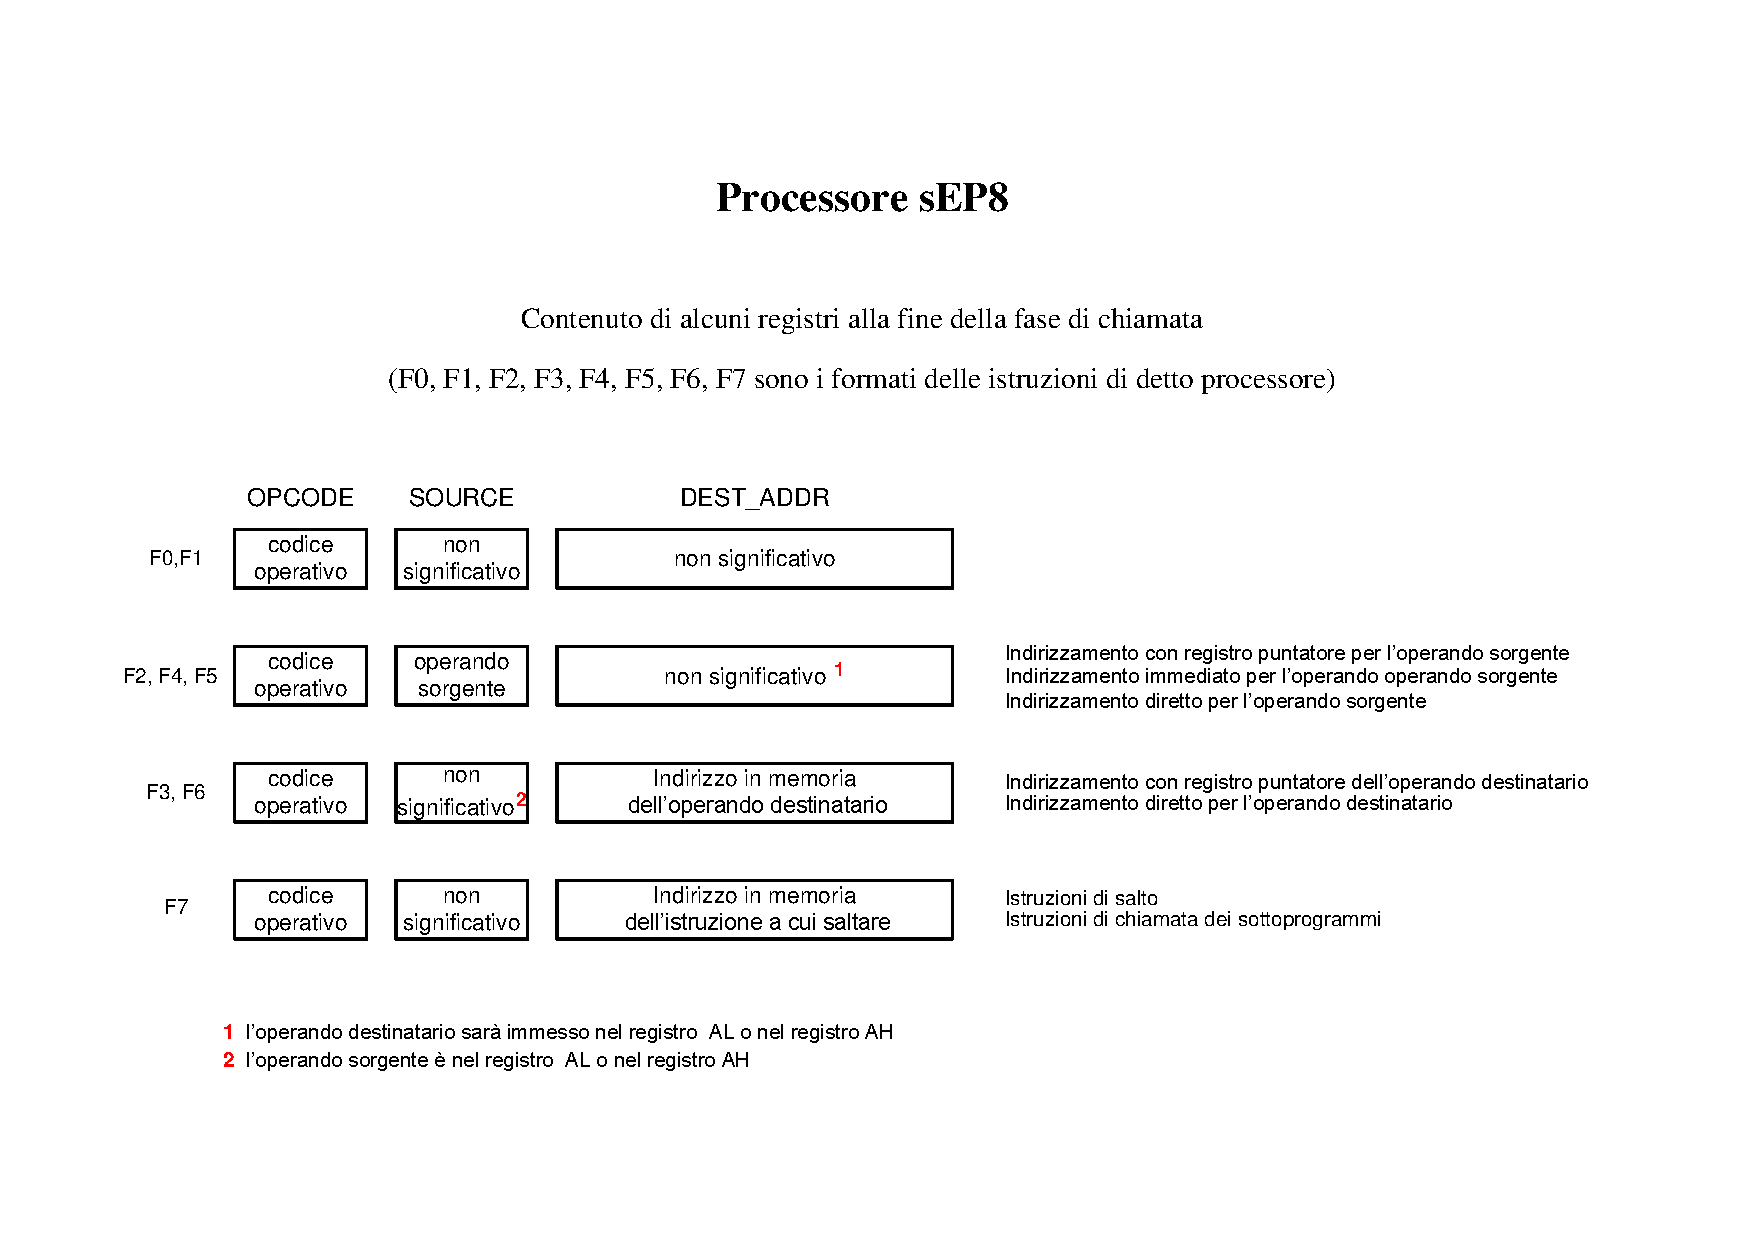
\includepdf[pagecommand={\thispagestyle{plain}},addtotoc={1,section,1,{Corsini - Registri processore sEP8 a seguito della fase di fetch},s2},landscape,scale=0.95,pages=-]{pdf/corsini4}
\section{Ricapitoliamo sugli stati della fase di fetch}
\small
Si tenga conto che al termine della fase di fetch avremo
\begin{itemize}
\item l'OPCODE nel registro OPCODE
\item L'operando sorgente nel registro SOURCE, se il sorgente è immediato o in memoria (e non è un registro)
\item L'operando destinatario nel registro DEST$\_$ADDR, se il destinatario è in memoria (e non è un registro)
\end{itemize}
\paragraph{Step}
\begin{itemize}
\item \textbf{fetch0}: Prendo l'indirizzo memorizzato nell'IP, incremento l'indirizzo memorizzato nell'IP (la cosa avviene in parallelo), indico col registro MJR che lo stato da richiamare più avanti è fetch1, avvio un'operazione di lettura del contenuto all'indirizzo appena estratto. Abbiamo ottenuto l'OPCODE.
\item \textbf{fetch1}: Memorizzo nel registro OPCODE il risultato dell'operazione di lettura (un byte memorizzato nel registro di supporto APP0).
\item \textbf{fetch2 e fetch3}: Utilizzo il registro MJR per gestire un salto a tante vie. Devo capire come ho gestito gli operandi, quindi quale formato ho adottato.
\item Gestisco il formato adottato:
\begin{itemize}
\item \textbf{F0}: si salta diretto a fetchEnd, abbiamo già gli operandi nel processore.
\item \textbf{F1}: si salta diretto a fetchEnd, rimandiamo la gestione degli operandi alla fase di esecuzione.
\item \textbf{F2}: eseguiamo un'operazione di lettura di un byte nell'indirizzo puntato dal registro DP. Si memorizza il risultato della lettura (posto in APP0) nel registro SOURCE.
\item \textbf{F3}: del destinatario non ci interessa il contenuto, ma solo l'indirizzo. Mi limito a copiare l'indirizzo puntato da DP nel registro DEST$\_$ADDR.
\item \textbf{F4}: l'operando sorgente è posto nel byte immediatamente successivo a quello dell'OPCODE. Svolgo un'operazione di lettura di un byte nella locazione successiva, e pongo il risultato della lettura nel registro SOURCE. Ovviamente incrementiamo IP una volta in più (ricordarsi che le istruzioni sono eseguite in parallelo, non in sequenza).
\item \textbf{F5}: l'operando sorgente è un indirizzo memorizzato su 3 byte successivi. Svolgo un'operazione di lettura su 3 byte (readM) per recuperare questo indirizzo. Dopo aver recuperato l'indirizzo (memorizzato in APP2, APP1, APP0) svolgo un'ulteriore operazione di lettura (su un byte) per recuperare il contenuto della locazione puntata dall'indirizzo. Pongo il risultato di quest'ultima lettura nel registro SOURCE.
\item \textbf{F6}: svolgo un'operazione di lettura su 3 byte, come prima, per recuperare l'indirizzo posto in modo diretto. Il risultato della lettura viene posto in DEST$\_$ADDR (ricordarsi che del destinatario ci interessa solo l'indirizzo, non il contenuto).
\item \textbf{F7}: le istruzioni di salto presentano solo l'operando destinatario. Svolgo un'operazione di lettura su 3 byte per recuperare l'indirizzo, come prima, e pongo come contenuto di DEST$\_$ADDR l'indirizzo appena estratto.
\end{itemize}
\item \textbf{fetchEnd e fetchEnd1}: conclusione della fase di fetch. Memorizzo nel registro MJR il risultato di una rete combinatoria. Questa restituisce il prossimo stato a cui saltare. Con questo salto concluso si passa alla fase di esecuzione dell'istruzione.
\end{itemize}
\normalsize

\chapter{Mercoledì 02/12/2020}
\desctotoc{\small\begin{itemize}
\item Fase di esecuzione.
\item Introduzione alle interfacce: descrizione di un'interfaccia a livello funzionale,  tipi di interfacce, necessità di introdurre meccanismi di handshake.
\end{itemize}\normalsize}
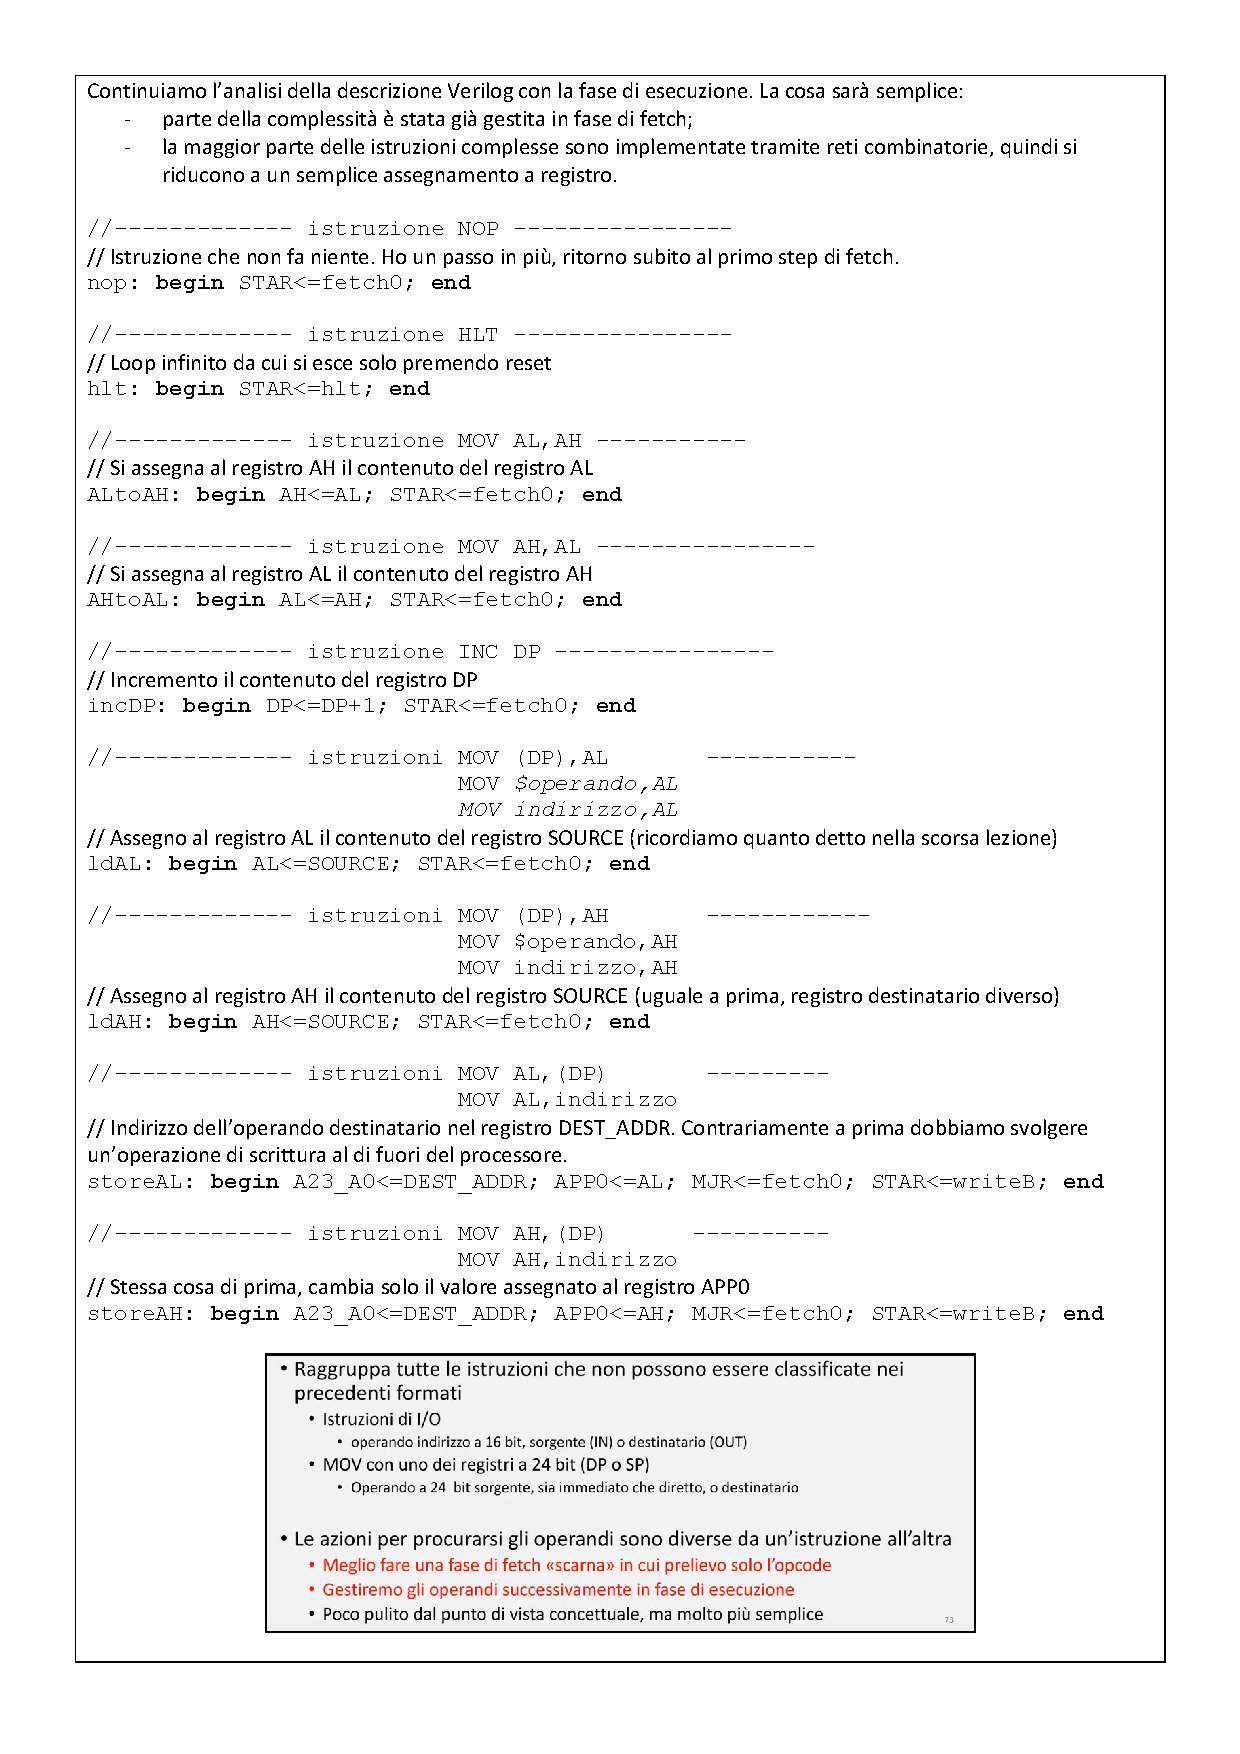
\includepdf[pagecommand={\thispagestyle{plain}},scale=0.92,pages=-]{pdf/calcolatore4}

\chapter{Giovedì 03/12/2020}
\desctotoc{\small\begin{itemize}
\item Interfaccia parallela di ingresso senza handshake.
\item Interfaccia parallela di uscita senza handshake.
\item Montaggio di interfacce parallele di ingresso e uscita.
\item Interfaccia parallela di ingresso con handshake: descrizione Verilog della RSS che gestisce l'handshake.
\item Interfaccia parallela di uscita con handshake: descrizione Verilog della RSS che gestisce l'handshake.
\item Interfaccia parallela di ingresso-uscita con handshake.
\item Interfacce seriali: nozioni di comunicazione seriale, descrizione Verilog di Trasmettitore e Ricevitore.
\end{itemize}\normalsize}
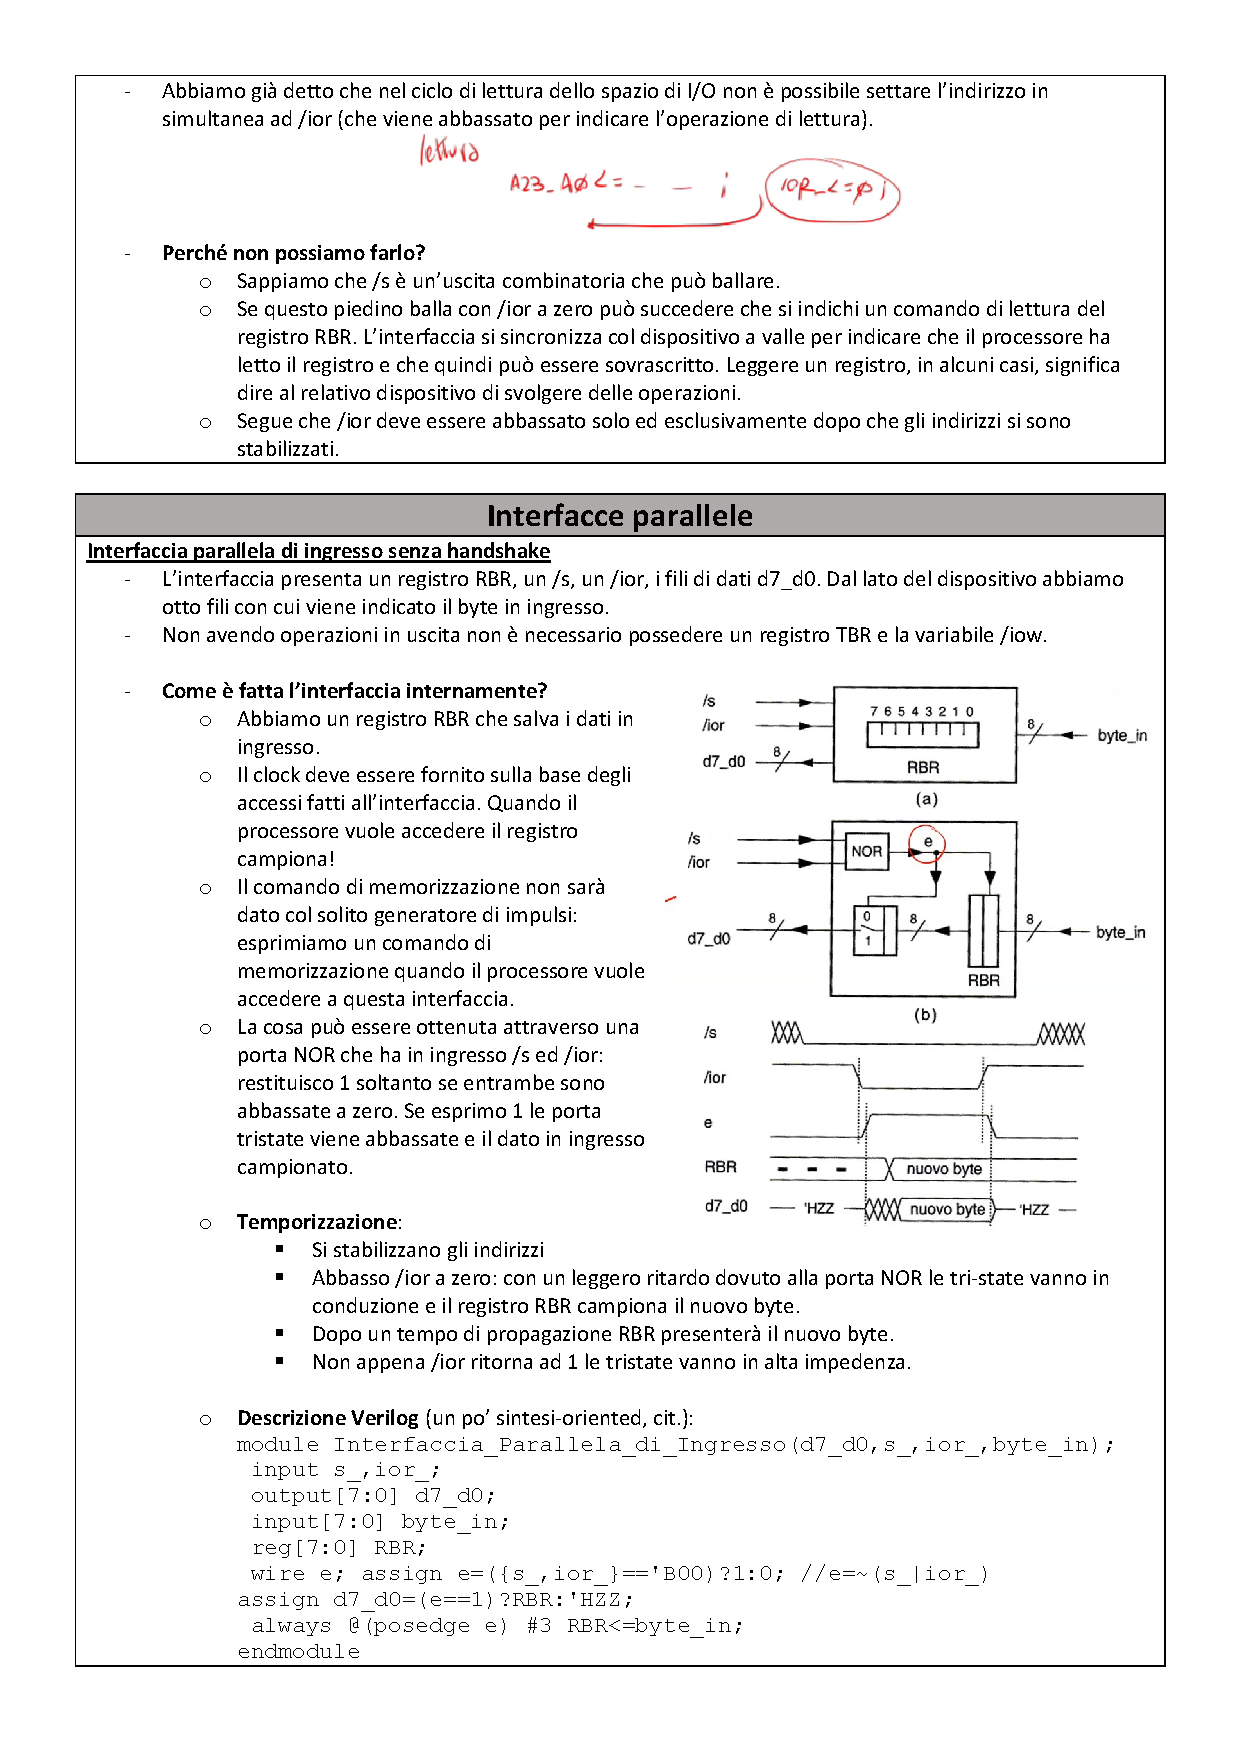
\includepdf[pagecommand={\thispagestyle{plain}},scale=0.92,pages=-]{pdf/calcolatore5}


\chapter{Martedì 09/12/2020}
\section{Conversione analogico/digitale e digitale/analogica}
Finora ci siamo limitati a osservare interfacce che consentono a due calcolatori di dialogare tra loro. Non dobbiamo farci ingannare dall'apparenza che i bit ci siano per magia: nel mondo esterno al calcolatore l'informazione è associata a grandezze analogiche, cioè grandezze che cambiano continuamente nel tempo (in contrapposizione alle stringhe di bit presenti nei calcolatori, che variano in modo discreto).  Abbiamo la necessità di svolgere le seguenti conversioni:
\begin{itemize}
\item \textbf{Conversione A/D}: conversione di grandezze analogiche in stringhe di bit (comunicazione del mondo esterno col calcolatore)
\item \textbf{Conversione D/A}: conversione di stringhe di bit in grandezze analogiche (comunicazione del calcolatore col mondo esterno).
\end{itemize}
La grandezza analogica da noi considerata è la \underline{tensione}.
\paragraph{Obiettivo}
\[\boxed{\text{\small Convertire una tensione $v$ in un numero $x$ (naturale o intero), in base 2 e rappresentato su $N$ bit, e viceversa}}\] 
Dove $N$ è solitamente 8 o 16. La tensione sta su una scala di FSR volts (\emph{Full-scale Range}): tipicamente abbiamo $\text{FSR} \in [5;30]$.
\paragraph{Interpretazione del numero o della tensione} Distinguiamo due tipi di conversioni:
\begin{itemize}
\item \textbf{Conversione unipolare}: $v \in [0;\text{FSR}]$ (tensioni positive), $x \in [0;2^N-1]$ (numeri naturali)
\item \textbf{Conversione bipolare}: $v \in \left[-\frac{\text{FSR}}{2};+\frac{\text{FSR}}{2}\right]$ (tensioni negative e positive),\\$x \in [-2^{N-1};2^{N-1}-1]$ (numeri naturali)
\end{itemize}
\paragraph{Mondo ideale} Definiamo il rapporto tra le due scale (tensione e numero)
\[K=\frac{\text{FSR}}{2^N}\]
in una conversione ideale dovrei ottenere 
\[v=K\cdot x\]
\paragraph{Mondo non ideale} Nella realtà questa cosa non è possibile poichè abbiamo un errore di conversione
\[|v-k \cdot x| \leq \text{err}\]
Questo errore è dovuto ai seguenti fattori:
\begin{enumerate}
\item \textbf{Imprecisioni circuitali}, cioè componenti di un circuito che non si comportano in maniera ideale. Questo errore, difficilmente eliminabile, è presente sia nella conversione D/A che in quella A/D. Si parla di \textbf{errore di non linearità}.
\item \textbf{Arrotondamento} (o \textbf{Errore di quantizzazione}). Si tenga conto nella formula $v=K\cdot x$ che $v \in \mathbb{R}$ e $x \in \mathbb{Z}$: questo significa che nella conversione A/D, cioè nel passaggio da tensione a numero, si avrà perdita di informazione (conversione da numero reale a numero intero).  
\end{enumerate}
\paragraph{Riflettiamo sull'errore di linearità} L'errore di linearità deve essere più piccolo di $\frac{K}{2}$. La presenza dell'errore ci porta a dire che la tensione appartiene a questo intervallo
\[v \in [K \cdot x - \text{err}; K \cdot x + \text{err}]\]
avere un errore chec non rispetta la condizione detta significa avere intervalli parzialmente sovrapposti, quindi convertire numeri più grandi in tensioni più piccole e viceversa.
\paragraph{Riflettiamo sull'errore di quantizzazione} Supponiamo di dividere la scala FSR in $2^N$ intervalli uguali a K, e di convertire tutto l'intervallo nello stesso numero.
\begin{center}
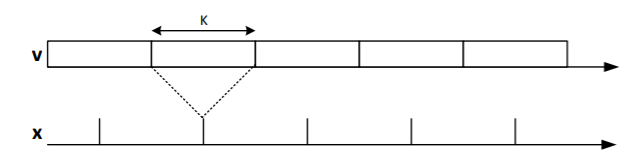
\includegraphics{img/232.PNG}
\end{center}
La conversione da $v$ a $x$ sarà esatta per la tensione al centro dell'intervallo, ed errata di $\pm \frac{K}{2}$ per le tensioni agli estremi.
\paragraph{Conclusioni}
\begin{itemize}
\item Nella conversione D/A dobbiamo avere $\text{err} < \frac{K}{2}$ (errore di non linearità)
\item Nella conversione A/D dobbiamo avere $\text{err} < \frac{K}{2}+\frac{K}{2}=K$ (errore di non linearità ed errore di quantizzazione)
\end{itemize}
\paragraph{Esempi di conversioni} Presenti degli esempi di conversione a pagina 53 della dispensa sulla struttura del calcolatore.
\paragraph{Tempi di risposta delle conversioni}
\begin{itemize}
\item I convertitori D/A sono circuiti estremamente semplici. Sono velocissimi (pochi ns).
\item I convertitori A/D hanno tempi di risposta variabili: sono circuiti sequenziali dove posso incontrare architetture diverse. I convertitori da noi considerati hanno tempi di risposta di qualche centinaio di ns.
\end{itemize}
\paragraph{Osservazione sulla conversione bipolare} I convertitori bipolari rappresentano i numeri interi con rappresentazione in traslazione. Il numero intero $x$ è rappresentato dal naturale
\[X=x+2^{N-1}\]
la tensione negativa di fondo scala, che corrisponde al numero intero negativo più piccolo, verrà convertita nel naturale 0. Ricordarsi che la conversione da traslazione a complemento a 2, e viceversa, si ottiene complementando il MSB.

\subsection{Convertitore D/A}
\begin{center}
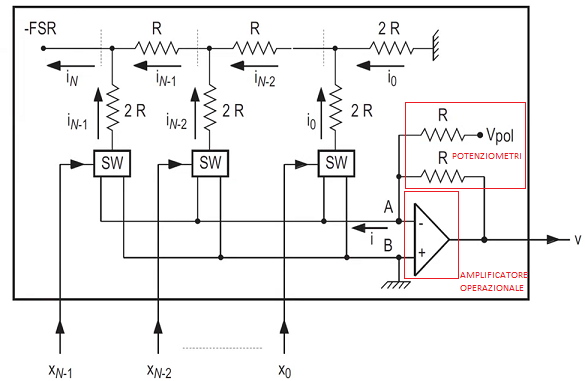
\includegraphics{img/233.PNG}
\end{center}
La tensione $v$ in uscita dovrà essere direttamente proporzionale al numero posto in ingresso (già da questo si capisce che la rappresentazione avviene per traslazione). Facciamo l'assunzione che tutte le linee verticali siano connesse a massa: provengono tutte da switch, che presentano in ingresso la linea A e la linea B. La linea B è esplicitamente connessa a massa, la linea A lo verificheremo prossimamente. 
\begin{itemize}
\item Ogni ramo verticale presenta la stessa corrente che scorre nel ramo orizzontale alla sua destra.
\item La resistenza vista a destra di ogni tratteggio è pari ad $R$. 
\item Ottengo due resistenze in serie che sommate mi danno $R+R=2R$.
\item La linea verticale immediatamente vicina al ramo orizzontale considerato presenta sempre come resistenza $2R$, quindi otteniamo in ogni filo verticale lo stesso risultato di prima.
\item Per quanto riguarda la corrente abbiamo, nel tratteggio vicino alla linea verticale più a destra
\[i_p=i_0+i_0=2\cdot i_k\]
\item Sommando le varie correnti otteniamo, alla fine,
\[\boxed{i_N=2^N \cdot i_0}\]
\end{itemize}
Osservando che $i_N=\frac{FSR}{R}$ troviamo
\[2^N \cdot i_0 = \frac{FSR}{R}\]
quindi
\[i_0=\frac{\text{FSR}}{2^N} \cdot \frac{1}{R}=\frac{K}{R}\]
dobbiamo ancora verificare che i rami verticali siano collegati a massa.
\paragraph{Vediamo gli switch} Gli switch sono guidati dai bit della rappresentazione del numero da convertire. Abbiamo tanti switch quante le cifre del numero.
\begin{itemize}
\item Se $x_j=0$ l'interruttore è connessa alla linea B, quindi a massa.
\item Se $x_j=1$ 'interruttore è connesso alla linea A, che non sappiamo quanto vale.
\end{itemize}
\paragraph{Amplificatore operazionale} Componente connessa all'alimentazione, la corrente non proviene dagli ingressi.
\[V^{\text{out}}=\alpha \cdot (V^+ - V^-)\]
con $\alpha >> 1$, la tensione dipende dalle differenze di tensione agli ingressi dell'amplificatore.
tenendo conto che il filo B è connesso a massa possiamo dire
\[V^{\text{out}}=- \alpha \cdot  V^-\]
Consideriamo anche l'altro ramo, quello con resistenza $R$ e corrente $i_a$
\[V^{\text{out}}-R \cdot i_a = V^-\]
unisco il tutto e ottengo
\[V^{\text{out}}=-\alpha \cdot V^{\text{out}} + \alpha \cdot R \cdot i_a\]
quindi
\[V^{\text{out}}=\frac{\alpha}{1+\alpha} \cdot R \cdot i_a \approx R \cdot i_a\]
questo mi permette di dire $V^- \approx 0$. $\qed$
\paragraph{Quanto vale la corrente che esce da A e va verso sinistra?} Tenendo conto di quanto detto sullo switch affermiamo che
\begin{align*}i&=x_0 \cdot i_0+ x_1 \cdot i_1 + \dots + x_{N-1} \cdot i_{N-1}\\&=i_0 \cdot x_0 + (2 \cdot i _0) \cdot x_1 + \dots + (2^{N-1} \cdot i_0) \cdot x_{N-1}=i_0 \cdot \sum_{i=0}^{N-1} 2^i \cdot x_i\end{align*}
ci siamo ricordati che $i_1=2 \cdot i_0$, e così via fino ad arrivare a $i_{N-1}= 2^{N-1} \cdot i_0$. La sommatoria ottenuta è la rappresentazione posizionale in base 2 di un numero naturale $X$. Ricordandomi che $i_0=\frac{K}{R}$ ottengo
\[i=\frac{K}{R} \cdot\sum_{i=0}^{N-1} 2^i \cdot x_i = \frac{K}{R}\cdot X\]
segue che gli switch alterano la corrente che scorre da $A$ verso sinistra.
\paragraph{Come faccio uscire la tensione giusta dal convertitore?} Scriviamo le equazioni di bilancio della corrente al nodo $A$
\[\frac{K}{R} \cdot X = \frac{V_{pol}+V}{R}\]
Mi sbarazzo di $R$ trovando
\[K \cdot X = V_{pol} + V\]
quindi (raccolgo rispetto a K)
\[V=K \cdot \left(X-V_{pol} \cdot \frac{2^N}{FSR}\right)\]
otteniamo che $V$ è proporzionale rispetto ad $X$. Segue che con
\begin{itemize}
\item $V_{pol}=0$ avrò una conversione unipolare $V= K \cdot X$, mentre con
\item $V_{pol}=\frac{FSR}{2}$ avrò una conversione bipolare
\[V=K \cdot (X- 2^{N-1})\]
cioè il numero rappresentato in traslazione in base 2.
\end{itemize}
Il circuito è in sostanza combinatorio. 
\paragraph{Problema 1: Situazione precedente nella realtà} Quanto spiegato poco fa è valido solo in un modello ideale. Nella realtà dobbiamo tener conto di errori. Riprendiamo l'equazione di bilancio e teniamo conto della cosa
\[\frac{K}{R} \cdot X = \frac{V_{pol}\cdot \gamma_1+V \cdot \gamma_2}{R}\]
otteniamo
\[V = \frac{K}{\gamma_2} \cdot \left(X-V_{pol} \cdot \gamma_1 \cdot \frac{2^N}{FSR}\right)\]
osserviamo il rapporto linea tra tensione e ingresso $X$ (sappiamo che esiste una proporzionalità diretta tra tensione in uscita e stringa di bit $X$ posta in ingresso)
\begin{itemize}
\item Se altero $\gamma_2$ altero la pendenza della retta.
\item Se altero $\gamma_1$ traslo la retta.
\end{itemize}
A tutto questo segue la necessità di dover tarare il convertitore prima di svolgere questa cosa. Le due resistenze vicine all'amplificatore operazionale sono dette \emph{potenziometri}, cioè resistenze variabili che possono essere tarate.
\paragraph{Problema 2: Variazioni a frequenza elevata} Supponiamo di voler passare da $X=01111111$ alla sua complementata $X=10000000$. Sappiamo fin dall'inizio che la rete non percepirà mai, in modo istantaneo e parallelo, la variazione di tutti i bit. Seguono stati intermedi. Questo comporta variazioni ad alta frequenza, un qualcosa che deve essere evitato. La soluzione è porre un filtro passa-basso, che taglia le variazioni a frequenza troppo elevata.

\subsubsection{Interfaccia per la conversione D/A} 
\paragraph{Attenzione} Non confondere il convertitore con l'interfaccia!
\begin{center}
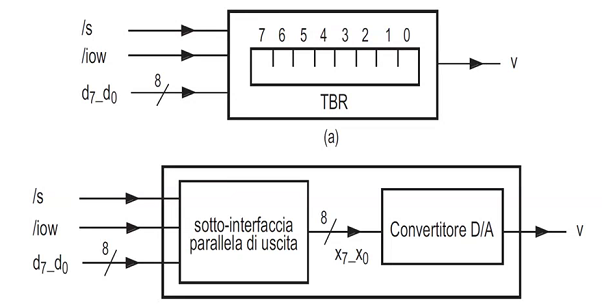
\includegraphics{img/234.PNG}
\end{center}
Abbiamo un'interfaccia parallela senza handshake, con un unico registro TBR (posto in una sotto interfaccia parallela di uscita) e un convertitore D/A. 
\paragraph{Velocità} Il convertitore D/A è molto più veloce del processore, quindi non servono ulteriori cose nell'interfaccia.

\subsection{Convertitore A/D}
\begin{center}
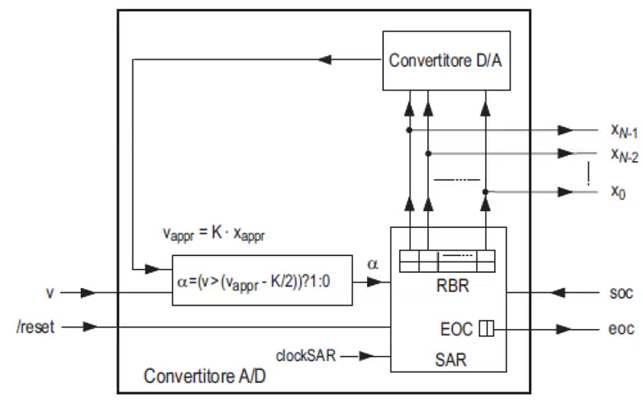
\includegraphics{img/235.PNG}
\end{center}
Il convertitore che andiamo a descrivere è detto \textbf{convertitore A/D ad approssimazioni successive} ad 8 bit. Il cuore del convertitore è la RSS detta SAR (\emph{Successive Approximation Register}). 
\begin{itemize}
\item All'interno del convertitore A/D è presente un convertitore D/A (chiaramente dovrò utilizzare un convertitore bipolare o unipolare in base alle circostanze) che utilizzerò per generare una tensione da confrontare, mediante comparatore analogico, con la tensione in ingresso.
\item Utilizzeremo un'handshake soc/eoc, considerando la mole di lavoro.
\item Il convertitore esegue una \textbf{ricerca logaritmica} (detta bisezione, o ricerca binaria).
\begin{itemize}
\item Ho una tensione $v$ analogica in ingresso, mantenuta costante nel corso dell'esecuzione dell'algoritmo mediante latch analogico (non avrebbe senso farla ballare durante i confronti, osservazione).
\item Quando il convertiitore percepisce $\text{soc}=1$ inizia a ``sparare'' numeri nel convertitore D/A. Si pone come primo numero quello al centro dell'intervallo di rappresentabilità ($100 \dots 00$). Questo numero è valido sia con conversione unipolare che con conversione bipolare: 
\item Ogni tensione ottenuta viene confrontata con la tensione in ingresso (resa costante, ricordiamo) con un comparatore di tensione.
\item Se la tensione generata è più grande della tensione in ingresso allora avremo $\alpha=1$, quindi la cifra considerata in una certa iterazione uguale ad $1$. 
\item Continuo a ripetere le operazioni precedenti, quindi a svolgere confronti tra tensioni.
\item Il numero di passi da svolgere è pari al numero di bit: ogni confronto, in base 2, mi permette di individuare un bit. Li determiniamo dalla cifra più significativa a quella meno significativa.
\end{itemize}
\end{itemize}
\paragraph{Esempio}
\begin{center}
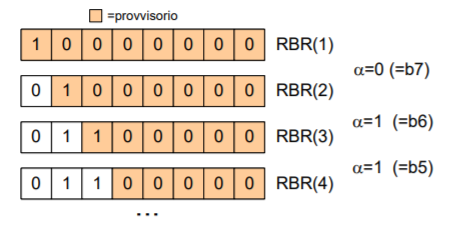
\includegraphics{img/236.PNG}
\end{center}
Vediamo l'esempio qua sopra. Ogni volta:
\begin{itemize}
\item Eseguo il confronto fra tensioni
\item Determino se settare o resettare la cifra. La cifra meno significativa immediatamente successiva viene impostata uguale ad 1.
\end{itemize}
\paragraph{Descrizione Verilog} Descriviamo la RSS che permette di gestire l'handshake e il contenuto del buffer che ogni volta sarà ``sparato'' verso il convertitore D/A.
\begin{verbatim}
module SAR(eoc,x7_x0,soc,alpha,clockSAR,reset_);
 input clockSAR,reset_;
 input soc,alpha;
 output eoc;
 output[7:0] x7_x0;
 reg EOC; assign eoc=EOC;
 reg[7:0] RBR; assign x7_x0=RBR;
 reg[3:0] STAR;
 parameter S0=0,S1=1,S2=2,S3=3,S4=4,S5=5,S6=6,S7=7,S8=8,S9=9,S10=10;
 
 always @(reset_==0) #1 begin EOC<=1; STAR<=S0; end
 always @(posedge clockSAR) if (reset_==1) #3
 casex(STAR)
 S0: begin EOC<=1; STAR<=(soc==0)?S0:S1; end
 S1: begin RBR<='B10000000; EOC<=0; STAR<=S2; end
 S2: begin RBR<={ alpha,'B1000000}; STAR<=S3; end
 S3: begin RBR<={RBR[7], alpha,'B100000}; STAR<=S4; end
 S4: begin RBR<={RBR[7:6],alpha,'B10000}; STAR<=S5; end
 S5: begin RBR<={RBR[7:5],alpha,'B1000}; STAR<=S6; end
 S6: begin RBR<={RBR[7:4],alpha,'B100}; STAR<=S7; end
 S7: begin RBR<={RBR[7:3],alpha,'B10}; STAR<=S8; end
 S8: begin RBR<={RBR[7:2],alpha,'B1}; STAR<=S9; end
 S9: begin RBR<={RBR[7:1],alpha }; STAR<=S10; end
 S10: begin EOC<=(soc==1)?0:1; STAR<=(soc==1)?S10:S0; end
 endcase
endmodule
\end{verbatim}
Si consideri anche la seguente versione, semplificata nel codice e nel numero di stati interni grazie all'introduzione di una function:
\begin{verbatim}
module SAR(eoc,x7_x0,soc,alpha,clockSAR,reset_);
 input clockSAR,reset_;
 input soc,alpha;
 output eoc;
 output[7:0] x7_x0;
 reg EOC; assign eoc=EOC;
 reg[7:0] RBR; assign x7_x0=RBR;
 reg[3:0] STAR;
 reg[2:0] COUNT;
 parameter S0=0,S1=1,S2=2,S3=3;
 
 always @(reset_==0) #1 begin EOC<=1; COUNT<=7; STAR<=S0; end
 always @(posedge clockSAR) if (reset_==1) #3
 casex(STAR)
 S0: begin EOC<=1; STAR<=(soc==0)?S0:S1; end
 S1: begin RBR<='B10000000; EOC<=0; STAR<=S2; end
 S2: begin RBR<=nuovobyte(RBR, alpha, COUNT); COUNT<=COUNT-1;
 STAR<=(COUNT==0)?S3:S2; end
 S3: begin EOC<=(soc==1)?0:1; STAR<=(soc==1)?S3:S0; end
 endcase
 
 function [7:0] nuovobyte;
 input [7:0] vecchiobyte;
 input alpha;
 input [2:0] posizione;
 casex (posizione)
 7: nuovobyte={ alpha,'B1000000};
 6: nuovobyte={vecchiobyte[7], alpha,'B100000};
 5: nuovobyte={vecchiobyte[7:6],alpha,'B10000};
 4: nuovobyte={vecchiobyte[7:5],alpha,'B1000};
 3: nuovobyte={vecchiobyte[7:4],alpha,'B100};
 2: nuovobyte={vecchiobyte[7:3],alpha,'B10};
 1: nuovobyte={vecchiobyte[7:2],alpha,'B1};
 0: nuovobyte={vecchiobyte[7:1],alpha };
 endcase
 endfunction
endmodule\end{verbatim}
\begin{itemize}
\item Ogni volta, sfruttando l'ingresso alpha generato dal comparatore, si determina un bit della sequenza di cifre. 
\item La sequenza memorizzata inizialmente nel RBR è provvisoria, quando alzeremo eoc il processore chiederà una lettura del buffer trovando la sequenza definitiva.
\end{itemize}

\subsubsection{Interfaccia di conversione A/D}
\paragraph{Ricordiamo di nuovo} L'interfaccia non è il convertitore.
\begin{center}
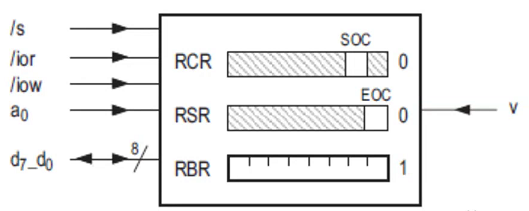
\includegraphics{img/237.PNG}
\end{center}
Abbiamo un'interfaccia parallela con handshake soc/eoc. Presenta i seguenti registri:
\begin{itemize}
\item Il registro di Buffer dove finisce il risultato (RBR, \emph{Receive Buffer Registry})
\item Un registro di stato per leggere il valore di eoc (RSR, \emph{Receive Status Registry})
\item Un registro di controllo per poter aggiornare il valore di soc (RCR, \emph{Receive Control Registry}).
\end{itemize}
Gli ultimi due indirizzi sono mappati allo stesso indirizzo logico (si ottiene il registro RSCR, \emph{Receive Status and Control Registry}). Non è un problema perchè i bit non si sovrappongono: inoltre la rete sa cosa restituire in base all'operazione indicata (lettura o scrittura).
\paragraph{Spogliamo l'interfaccia}
\begin{center}
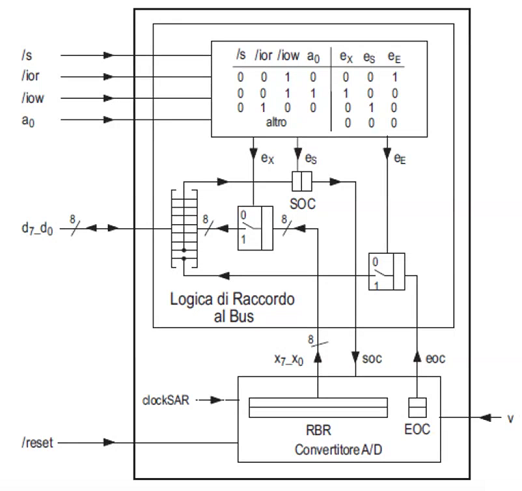
\includegraphics{img/238.PNG}
\end{center}
\begin{itemize}
\item Le operazioni possibili sono:
\begin{itemize}
\item lettura di eoc
\item letture di RBR
\item scrittura di soc
\end{itemize}
\item Abbiamo una rete combinatoria che permette di gestire le porte tristate (e il registro SOC). Osserviamola:
\begin{itemize}
\item Quando le variabili di pilotaggio non indicano una particolare operazione tutte le porte sono in alta impedenza.
\item Quando voglio leggere eoc avrò $e_E=1$, quindi la porta relativa in conduzione. L'utente troverà eoc sul filo in posizione 0 (nei fili di dati).
\item Quando voglio leggere RBR avrò $e_x=1$, enabler di tante porte tristate quante il numero di bit del registro (8). Tutte queste porte sono in conduzione, le rimanenti in alta impedenza. L'utente troverà in uscita, su tutti i fili di dati, il valore del registro RBR.
\item Quando voglio scrivere su soc avrò $e_S=1$. Questa variabile è il clock per il registro SOC: se $e_s=1$ il valore del registro impostato sarà quello posto in posizione 1 (nei fili di dati). Segue un nuovo ingresso nella SAR e quindi l'inizio di una nuova operazione di conversione, se necessario.
\end{itemize}
\end{itemize}
\appendix
\part{[Extra] Riassunto su interruzioni e protezioni dal libro di Corsini}
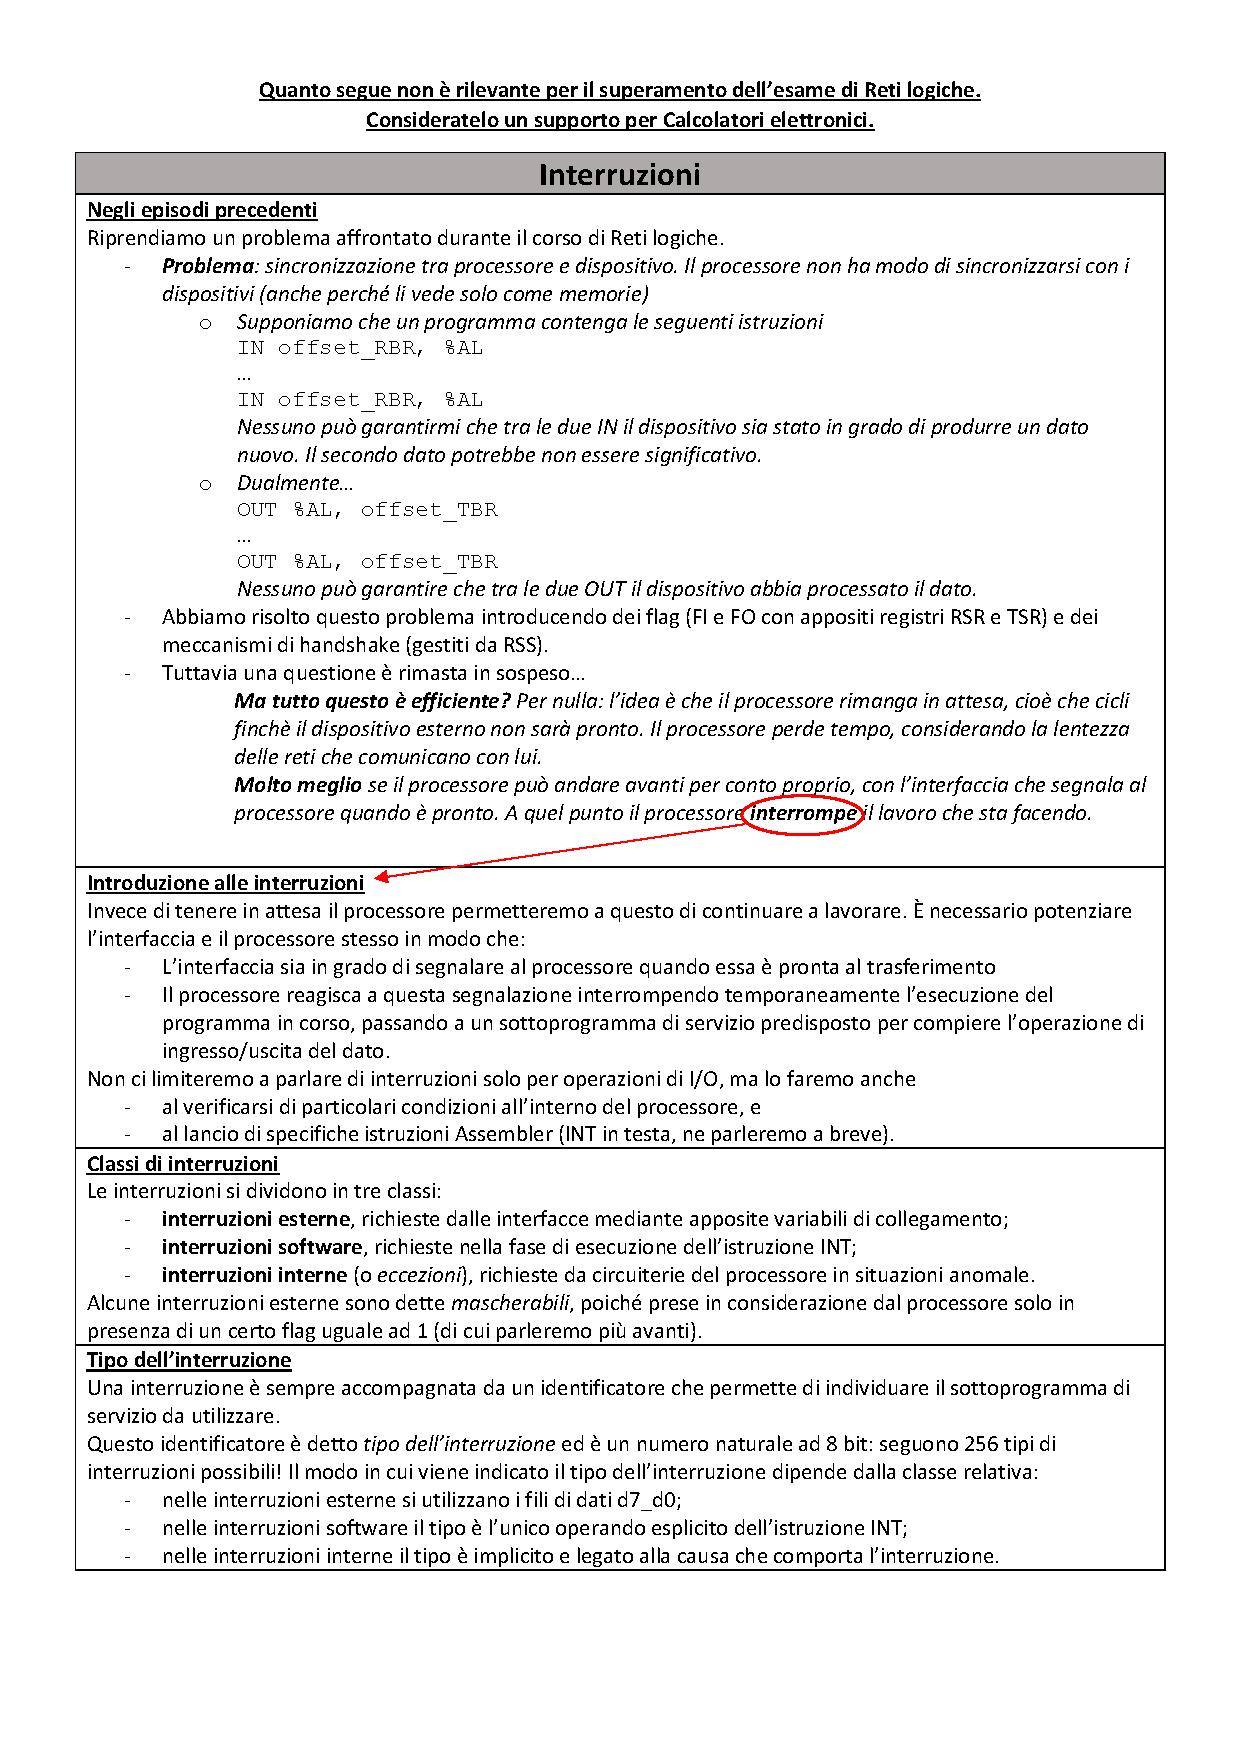
\includepdf[pagecommand={\thispagestyle{plain}},scale=0.92,pages=-]{pdf/pdfextra}
\end{document}
